\section{Pattern Analysis}

\begin{frame}{Pattern Analysis with EOF}
  \begin{columns}
    \begin{column}{.5\textwidth}
      \begin{itemize}
        \item For those familiar: it is related to PCA
        \item very widely used in geospatial sciences (see review paper from \citeauthor{hannachi_empirical_2007} \cite{hannachi_empirical_2007})
        \item can be used for dimensionality reduction, filtering, pattern recognition \dots
        \item already been used for IVT fields (\citeauthor{ayantobo_integrated_2022} \cite{ayantobo_integrated_2022})
%        \item also some interesting modifications: REOFs
      \end{itemize} 
      
    \end{column}
    \begin{column}{.5\textwidth}
    \begin{figure}[t]
      \centering
      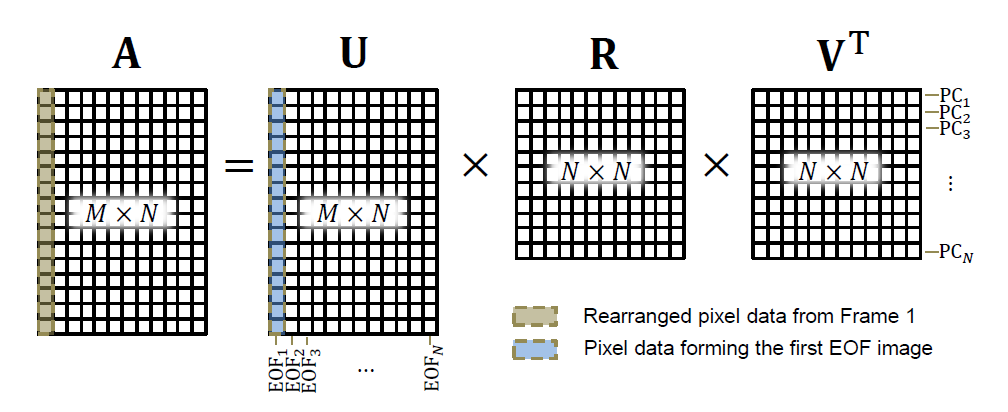
\includegraphics[width=\columnwidth]{imglib/svd_matrices.png}
      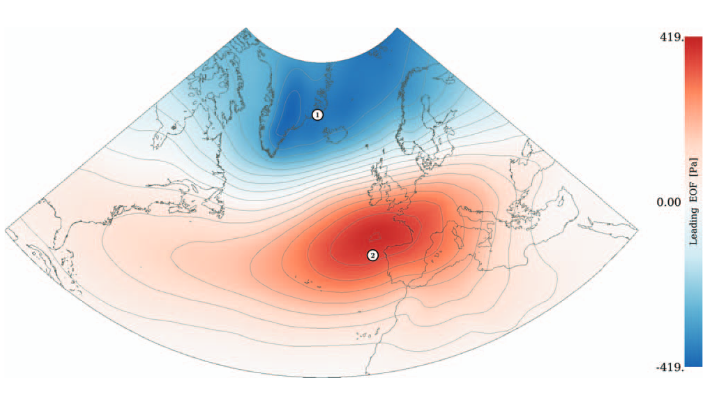
\includegraphics[width=.7\columnwidth]{imglib/nao_eof_index.png}
    \end{figure}

    \end{column}
    
  \end{columns}
\end{frame}

\begin{frame}{My current plan}

  \begin{enumerate}
    \item Generate an IVT field from the MPI-GE
    \item Implement a similar windowed EOF approach as \cite{vietinghoff_visual_2021} to track changes in moisture transport patterns
      \begin{itemize}
        \item maybe also implement/use some other analyses from similar work 
      \end{itemize}
    \item Visualize the uncertain Scalar Fields over time
  \end{enumerate}
  
\end{frame}
